
%
%% Language setting
%% Replace `english' with e.g. `spanish' to change the document language
%\usepackage[english,russian]{babel}
%\usepackage{multirow}
%
%% multicol package
%\usepackage{multicol}
%\usepackage{ragged2e}
%
%% page number
%\usepackage{fancyhdr}
%\pagestyle{fancy}
%
%\fancyfoot[L]{\textbf{56}}
%\fancyfoot[R]{} 
%\fancyfoot[C]{} 
%
%\renewcommand{\headrulewidth}{0pt} % Убираем линию вверху страницы
%\renewcommand{\footrulewidth}{0pt} % Убираем линию внизу страницы
%
%
%% Set page size and margins
%% Replace `letterpaper' with `a4paper' for UK/EU standard size
%\usepackage[letterpaper,top=4cm,bottom=2cm,left=3.95cm,right=4.5cm,marginparwidth=1.75cm]{geometry}
%
%% Override Figures' ref. names
%\usepackage{graphicx}
%\makeatletter
%\renewcommand{\p@figure}{рис.\ }
%\makeatother
%
%% Math set letters
%\usepackage{amssymb}
%
%% Override Figures' captions
%\usepackage{subcaption}
%\DeclareCaptionLabelFormat{custom}{рис. 1}
%\DeclareCaptionLabelSeparator{custom}{ --- }
%\captionsetup
%{
%    labelformat=custom,
%    labelsep=custom
%}
%
%% Add Bibliography to contents
%\usepackage[nottoc,notlot,notlof]{tocbibind}
%
%% Other useful packages
%\usepackage{amsmath}
%\usepackage[colorlinks=true, allcolors=black]{hyperref}
%\usepackage{mathtools}% http://ctan.org/pkg/mathtools
%\usepackage[absolute,overlay]{textpos}

%\begin{document}
%\usepackage[letterpaper,top=4cm,bottom=2cm,left=5cm,right=5cm,marginparwidth=1.75cm]{geometry}

%\usepackage[letterpaper,top=2cm,bottom=2cm,left=77mm,right=2cm,marginparwidth=1.75cm]{geometry}

\begin{multicols}{3}
\RaggedRight
\setlength{\parskip}{0pt}
\setlength{\parindent}{0pt}
американский математик Д. Риордан в своей книге
«Введение в комбинаторный анализ» (М., ИЛ, 1963) как раз 
применяет термин «ладейный многочлен»! Чем это вызвано?

\setlength{\parindent}{17pt} 
Оказывается, большой класс комбинаторных задач сводится к определению
числа размещений на шахматной доске заданного числа ладей,
не угрожающих друг другу (ни одна пара ладей не должна
находиться на одной вертикали или горизонтали). А при
рассмотрении еще более сложных задач существенную роль игрет
многочлен 
{\setlength{\abovedisplayskip}{6pt}
\setlength{\belowdisplayskip}{6pt}
\[
\begin{aligned}
    R(x) &= r_0 + r_1x + \\
         &\phantom{=} r_2x^2 + \dots + \\
         &\phantom{=} r_kx^k + \dots + r_nx^n
\end{aligned}
\]} где \(r_k\) - число размещений на доске размера \(nxn\) не угрожающих друг другу \(k\)
ладей \((k = 0,1,2,...)\). Этот многочлен и был назван Риорданом ладейным; как мы видим,
такое название вполне оправдано.

Заметим, что бездонное море задач и проблем возникает тогда, когда речь заходит о
создании машины, играющей в шахматы (а точнее, программы для нее).

Этой модной в наши дни теме посвящены десяти и сотни специальных статей, книг, дискуссий и даже диссертаций, и мы не станем подробно останавливаться на ней.

% !!! column 1 END

\quad \\

\begin{flushleft}
\textbf{56}    
\end{flushleft}


\columnbreak

% !!! column 2 START

\begin{center}
  \textbf{От персидского шаха до наших дней}
\end{center} 

Наш разговор естественнее всего начать с рассмотрения свойств шахматной доски,
пока не расставляя на ней фигур.

Конечно, каждый из вас слышал знаменитую легенду о происхождении шахмат. Мудрец, придумавший их, потребовал в награду от персидского шаха, которому игра очень понравилась, столько зерен пшеницы, сколько понадобится для покрытия всех клеток шахматной доски, если на ее первую клетку положить одно зерно, а на каждую следующую вдвое больше, чем на предыдущую. (рис. 1)

\begin{flushleft}
    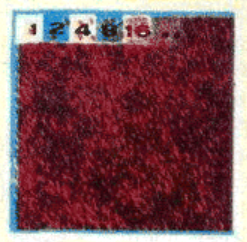
\includegraphics[width=\linewidth]{img1.png}
\end{flushleft}

\begin{flushleft}
Рис. 1.
\end{flushleft} 


Оказалось, что для этого не хватит пшеницы, хранящейся не только в амбарах персидского
шаха, но и во всех амбарах мира. Мудрец скромно потребовал
\begin{flushleft}
\(1 + 2 + 2^{2} + 2^{3} + ...\)
\(.. + 2^{63} = 2^{64} - 1\)
\end{flushleft}
зерен. Это число записывается двадцатью цифрами и превышает 18 квантиллионов \((2^{10}=\)

% !!! column 2 END

\columnbreak

% !!! column 3 START

\noindent \(=1024 \approx 10^{3})\). Конечно, с математикой здесь небольшая связь,
скорее, полученный результат как бы символически иллюстрирует грандиозные
математические возможности, скрывающиеся в шахматной доске.

Пожалуй, самое любопытное свойство шахматной доски заключается в том, что кратчайшее
расстояние на ней измеряется не обзятельно по прямой. Например, геометрическая расстояние от поля \(al\) до поля \(h8\) больше, чем до \(a8\), а королю на любой
из этих переходов потребуется ровно \(7\) ходов. Для математиков, которым
приходится сталкиваться с самыми разнообразными расстояниями (метриками), это обычное дело.

Особенно эффектно указанное свойство проявляется в знаменитом этюде Рети (рис. 2).

Кажется, совершенно нвероятным, что в этом плолжении белый король в состоянии догнать черную пешку.

\begin{flushleft}
    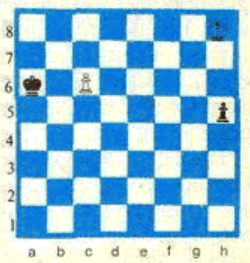
\includegraphics[width=\linewidth]{img2.png}
\end{flushleft}

\begin{flushleft}
Рис. 2. Р. Рети, 1921 г. 
Ничья.
\end{flushleft} 
Однако это становится возможным, если он

% !!! column 3 END

\end{multicols}